\subsection*{Blobs}\label{sec:blobs}
En blob er en sammenhængende region af pixels, der enten er betydeligt lysere eller mørkere end dens omgivelser, altså strukturer, der står i kontrast til deres baggrund. En blob kan derfor udvælges som værende et lokalt ekstrema i billedet.
I figur \ref{fig:lindblob} ses tre lyse blobs, på en mørk baggrund, illustreret som bakketoppe. Der hvor bakkerne mødes, eksistere et punkt, hvor dets hældning krummer op i en retning og krummer ned i en anden. Et sådant punkt kaldes et sadel-punkt. Et sadel-punkt er derfor ikke et ekstrema, og derfor ikke en blob.
\begin{figure}[H]
    \centering
    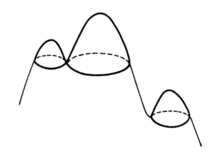
\includegraphics[width=0.35\textwidth]{fig/44.png}
    \vspace{-0.5em}   
    \begin{center}
    \caption{\textcolor{gray}{\footnotesize \textit{
    Tre lyse blobs på en mørk baggrund illustreret i 2 dimensioner \cite{blob}}}}
    \label{fig:lindblob}
     \end{center}
  \end{figure}
       \vspace{-2.7em}
\noindent
En blob kan udvælges ved at identificere den geometriske struktur i om omkring et punkt. De to principale krumninger i et punkt angiver, hvor meget overfladen bøjer i de forskellige retninger. Da et ekstrema angiver en blob, vil fortegnet for de to principale krumninger være ens. For et punkt placeret på et maksima vil de principale krumninger være konkave (nedadgående) og for et punkt placeret på et minima vil de principielle krumninger være konvekse (opadgående). For et punkt placeret på et saddle-point, vi den ene krumning være konkav og den anden konveks. \\ 
Om et punkt i billedet er placeret på et maksima, minima eller saddle-point, kan determineres ved en 'to variabel, anden-afledte-test'. Dette udføres ved at opstille en matrice, for et givent punkt, der indeholder dens dobbeltafledte i $x, y \text{ og } xy$ retningen også kaldet Hessian matricen $\mathcal{H}$.
\begin{equation}
\mathcal{H} = 
 \begin{bmatrix}
 	L_{xx} & L_{xy} \\
 	L_{xy} & L_{yy}
 \end{bmatrix}
 \label{hessianmatrixblob}
\end{equation}
hvor den andenafledte i $x$ retningen defineres ved:
\begin{equation}
L_{xx}(x, \sigma) = (\frac{\partial^2 }{\partial x^2 } G(x,y,\sigma)) * I
\label{lxx}
\end{equation}
Egenvektorerne for $\mathcal{H}$ beskriver retningerne af de principale krumninger af et punkt, hvor egenværdierne beskriver størrelserne af disse krumninger. Den geometriske struktur kan derved defineres ud fra Hessian matricens egenværdier $\lambda_1, \lambda_2$:
\begin{equation}
\begin{split}
indikator = 
\begin{cases}
\text{Minima} & \text{hvis } \lambda_1, \lambda_2 > 0, \\
\text{Maksima}& \text{hvis } \lambda_1, \lambda_2 < 0,  \\
\text{Sadel-Punkt} & \text{hvis } \lambda_1 \lambda_2 < 0.
\end{cases}
\end{split}
\label{maxsurp}
\end{equation}
En måde at estimere egenværdiernes fortegn, er ved at tage determinanten af hessian matricen:
\begin{equation}
\textbf{det}\mathcal{H} = L_{xx}L_{yy}-L_{xy}^2
\label{detofhessian}
\end{equation}
Da $\bold{det}(\mathcal{H})=\lambda_1 \lambda_2$ vil fortegnet af determinanten angive om et punkt er et ekstrema eller et sadel-punkt. Figur \ref{fig:makssad} illustrere, hvordan Hessian matricen approksimere den geometriske struktur i billedet med et andengradspolynomium. Figuren viser approksimeringen, med et punkt lokaliseret på et maksima og et saddle-point.
\begin{figure}[H]
    \centering
    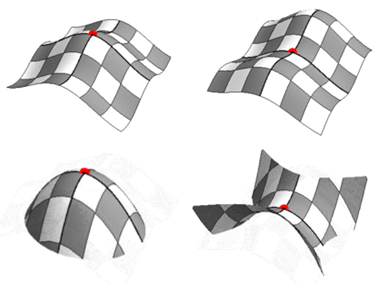
\includegraphics[width=0.50\textwidth]{fig/41.png}
    \vspace{-0.5em}
    \begin{center}
    \caption{\textcolor{gray}{\footnotesize \textit{
d   }}}
    \label{fig:makssad}
     \end{center}
  \end{figure}
       \vspace{-2.7em}
\noindent
En anden metode at detektere blobs er ved Laplace operatoren, som giver et stærkt filtersvar i centeret af en blob. Laplace operatoren kan defineres ved:
$$
\nabla^2L(x,y) = L_{xx}+L_{yy}
$$
Da laplace operatoren svarer til sporret af Hessian matricen $\bold{Tr}(\mathcal{H}) = \lambda_1 + \lambda_2$, vil filtersvaret fra laplace operatoren $\nabla^2L$ fortælle noget om egenværdierne. Et negativt respons, vil angive et maksima da egenværdierne begge vil være negative. Et positivt respons vil angive et minima da egenværdierne begge vil være positive.
\begin{equation}
\begin{split}
\text{indikator} = 
\begin{cases}
\text{Maksima}& \text{hvis } \nabla^2L < 0,  \\
\text{Minima} & \text{hvis } \nabla^2L > 0.
\end{cases}
\end{split}
\label{laplaceblob}
\end{equation}
Anvendes Laplace operatoren på Gaussfunktionen (ligning \eqref{2dgaussian}), kan resultatet diskretiseres og anvendes som en kerne, der kan foldes med et billede for identifere forekomster af blobs.
\begin{equation}
LoG= \nabla^2 G
\label{lap}
\end{equation}
Ved oprettelse af et skalarum udglattes billedet til grovere strukturer. 
Skal strukturer udpeges på tværs af skalaer, vil det være naturligt at udvælge lyse/mørke pletter (blobs), da de vil korrelere nogenlunde i placering og struktur. Dette skyldes blobbens sammenhængende struktur, der gør dem stabile over et større skalainterval. Som nævnt vil et stort filtersvar (postivit eller negativt) til Laplace operatoren definere en blob. Dette er dog kun tilfældet, hvis størrelsen af Laplace Gauss filteret svarer til størrelsen af blobben. En tilgang er at systematisk forøge størrelsen af Laplace Guass filteret for det eksisterende skalarum, og udvælge skalaen, hvor der afgives et maksimalt respons. Figur \ref{fig:laprespons} illustrere et filtersvar for en blob af konstant størrelse, udsat for stigende størrelser af et Laplace Gauss filter. Det ses at når blobben er betydeligt større en filteret, opfattes blobben som to kanter. Når størrelsen på filteret forøges, afgives et stort filtersvar, hvorefter når filterstørrelsen forøges yderligere, flades filtersvaret ud.
\begin{figure}[H]
    \centering
    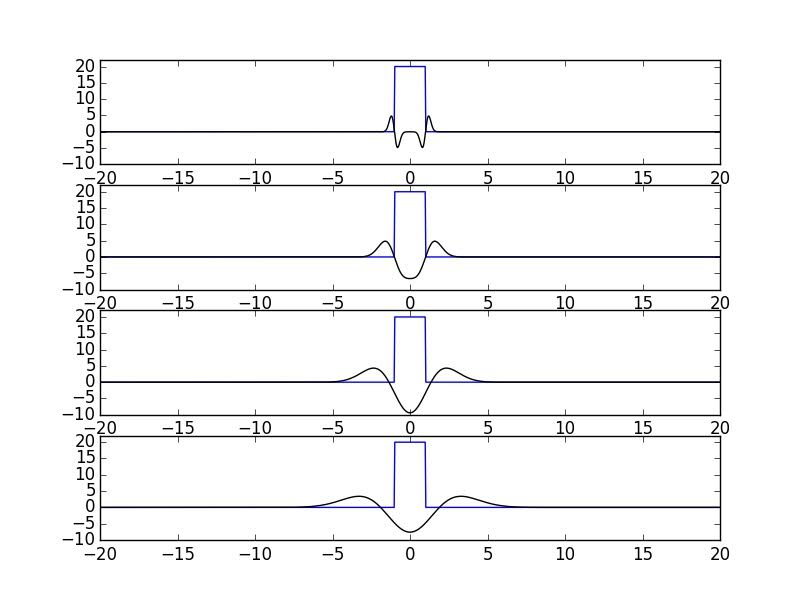
\includegraphics[width=0.80\textwidth]{fig/42.jpg}
    \vspace{-0.5em}
    \begin{center}
    \caption{\textcolor{gray}{\footnotesize \textit{En blob (den lysseblå firkant) udsat for et Laplace Gauss filter af stigende filterstørrelser.
}}}
    \label{fig:laprespons}
     \end{center}
  \end{figure}
       \vspace{-2.7em}
\noindent
En egenskab ved skalapræsentationen er at amplituden af de rumlige afledte vil falde. Dette er, som nævnt i sektion \ref{sec:scale}, grundet at maksima over skala ikke vil forøges og minima ikke formindskes. Amplituden af ekstremaer vil derfor altid formindskes over skala \cite{phdlind}. Dette resultere i at filtersvaret for $LoG$, vil formindskes når skalaparametren øges. For at muliggøre en sammenligning af filtersvaret over skala normaliseres filtersvaret ift. skala.  Lindenberg \cite{lindenscale} viser at ved anvendelse af billedets afledte af orden $p$, skal skalanormalisering ske ved at multiplicere filtersvaret med $\sigma^p$. Da $LoG$ anvender de andenafledte af et Gauss filter, multipliceres responset med $\sigma^2$. En skalanormaliseret Laplacian of Gauss, kan derfor opskrives som:
$$\sigma^2 \nabla^2G = \sigma^2(L_{xx}+L_{yy})$$ 